
At a high level each attack graph based security metric follows the simplified processing pipeline shown in Fig \ref{fig:metric_pipeline}. 

% \begin{table}[ht]
% \centering
% \caption{Generalized Metric Pipeline}
% \label{tab:metric_proc_pipeline}
% \resizebox{.48\textwidth}{!}{%
% \toprule
% \begin{tabular}{@{}p{.20\linewidth}p{.22\linewidth}p{.22\linewidth}p{.22\linewidth}@{}}
%  1. Input & 2. Pre-Process & 3. Compute  & 4. Report \\ \midrule
%  System Model & Generate AG & Measurement &  Return values \\
% \bottomrule
% \end{tabular}
% }
% \end{table}

\begin{figure*}[ht]
\centering
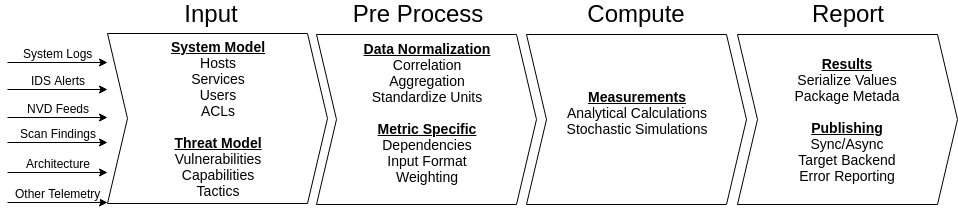
\includegraphics[width=.8\linewidth]{img/metric_calc_pipeline.png}
\caption{General Security Metric Evaluation Pipeline}
\label{fig:metric_pipeline}
\end{figure*} 

In Step 1, the inputs include host definitions, accounts and permissions, network connectivity and ACLs, system policies, vulnerability definitions, etc. It is usually assumed these parameters are collected through standard management tools and translated into a common system model for consumption by the attack graph generation engine. 

In Step 2, the system model is examined for policy violations or possible exploits that would lead to a given target's compromise. If a compromise is possible, an attack graph is produced. This is the expected input for most of the metrics we have examined, although some also assume the edges have been weighted with CVSS scores first.

The algorithm for computing the metric is run in step 3 with the attack graph as input, and the computed result is returned in the final step. 

Our first observation is that survivorship bias\cite{Wald_1980} is implicit in all AG based security metrics. An attack graph is produced \textit{only} when a system model includes in its definition enough detail to identify possible attacks. An attack graph will \textbf{not} be created if a system is totally \textit{secure}. Secure and insecure systems should, in theory at least, be mutually exclusive and collectively exhaustive; unfortunately, an attack graph will also \textbf{not} be created if a system is totally \textit{insecure}, but the system model or processing logic is incomplete. So, when validating AG metrics, we must have accepted a priori the selection bias inherent with their use. That is, we are not measuring if a system is secure or not; rather, we are measuring just how insecure that system is. 

With this in mind, validation can be seen as a test of how well a metric captures the scale of insecurity which is known to be on the system under test. We propose here a simple methodology for calibrating a metric and gauging it's accuracy in a controlled manner. 

\begin{algorithm}
\caption{Calibrate Weighted Security Metric}
\label{alg:calibrate_secmet}
\begin{algorithmic}
\REQUIRE Valid Attack Graph, N = \# partitions
\FOR{n $\in$ range (1..N)} 
 \STATE Fix all weights at $\frac{scale}{n}$ 
 \STATE Take measurement
\ENDFOR
 \end{algorithmic}
\end{algorithm}

What we assume in Algorithm \ref{alg:calibrate_secmet} is that the security metric is using some weighting scheme to influence an attacker's selection of paths, which is common in all but the structural metrics (more on these later) we've encountered. So, for CVSS base score weighted AG metrics, we would fix all vulnerabilities at the lowest score (1 in this case) and calculate the metric, and do the same again fixing all vulnerabilities at the highest score for the scale (10 for CVSS). This bounds the range of the metric under test. Creating more than 2 partitions of the score range gives us insight into the behaviour of the metric for this particular attack graph. An example of this calibration is given in \ref{sec_results}

To turn this testing algorithm into a benchmark, we need attack graphs which represent typical deployment scenarios. By far the most common use cases in the literature are small enterprise systems consisting of a limited number of distinct node types (web server, database, firewall, workstation, ...) and a 2-dimensional perimeter. While these examples are easily digestible when describing the applicability of an intensive mathematical derivation, they fall short of validating the new metric as it would be seen in the wild. We propose a standard benchmark set of attack graphs which isolate interesting attack patterns for study. In this way we can target \textit{micro-benchmarks} for specific properties, and integrate or compose models for a more rounded workload examination.

\begin{table*}[ht]
\centering
\caption{AG Standard Set - Target Scenarios}
\label{tab:ag_standard_set}
\begin{tabular}{@{}p{.15\linewidth}p{.15\linewidth}p{.15\linewidth}p{.15\linewidth}p{.15\linewidth}@{}}
\toprule
 & Enterprise & MEC/MANET &  Core &  Cloud \\ \midrule
Small (10-20) & Multi Site & UE Access  & Attachment Point & API misuse \\
Medium (100-200) & Container/K8s & 4G/5G & Layer 1\&2 & Hypervisor  \\
Large (1000-2000) & Insider/Exfil  &  IoT &  SDN/NFV & APT  \\ \bottomrule
\end{tabular}
\end{table*}

